\ours's OS-inspired multi-level memory architecture delineates between two primary memory types: \textbf{main context} (analogous to main memory/physical memory/RAM) and \textbf{external context} (analogous to disk memory/disk storage). 
Main context consists of the LLM \emph{prompt tokens}---anything in main context is considered \emph{in-context} and can be accessed by the LLM processor during inference.
External context refers to any information that is held outside of the LLMs fixed context window.
This \emph{out-of-context} data must always be explicitly moved into main context in order for it to be passed to the LLM processor during inference.
\ours provides function calls that the LLM processor to manage its own memory without any user intervention.

\subsection{Main context (\emph{prompt tokens})}

The prompt tokens in \ours are split into three contiguous sections: the \textbf{system instructions}, \textbf{working context}, and \textbf{FIFO Queue}. The system instructions are read-only (static) and contain information on the \ours control flow, the intended usage of the different memory levels, and instructions on how to use the \ours functions (e.g. how to retrieve out-of-context data). Working context is a fixed-size read/write block of unstructured text, writeable only via \ours function calls. In conversational settings, working context is intended to be used to store key facts, preferences, and other important information about the user and the persona the agent is adopting, allowing the agent to converse fluently with the user.
The FIFO queue stores a rolling history of messages, including messages between the agent and user, as well as system messages (e.g. memory warnings) and function call inputs and outputs. The first index in the FIFO queue stores a system message containing a recursive summary of messages that have been evicted from the queue.

\subsection{Queue Manager}

The queue manager manages messages in \textbf{recall storage} and the \textbf{FIFO queue}. When a new message is received by the system, the queue manager appends the incoming messages to the FIFO queue, concatenates the prompt tokens and triggers the LLM inference to generate LLM output (the completion tokens). The queue manager writes both the incoming message and the generated LLM output to recall storage (the \ours message database). When messages in recall storage are retrieved via a \ours function call, the queue manager appends them to the back of the queue to reinsert them into the LLM's context window.

The queue manager is also responsible for controlling context overflow via a queue eviction policy. When the prompt tokens exceed the `warning token count` of the underlying LLM's context window (e.g. 70\% of the context window), the queue manager inserts a system message into the queue warning the LLM of an impending queue eviction (a `memory pressure` warning) to allow the LLM to use \ours functions to store important information contained in the FIFO queue to working context or \textbf{archival storage} (a read/write database storing arbitrary length text objects). When the prompt tokens exceed the `flush token count' (e.g. 100\% of the context window), the queue manager flushes the queue to free up space in the context window: the queue manager evicts a specific count of messages (e.g. 50\% of the context window), generates a new recursive summary using the existing recursive summary and evicted messages. Once the queue is flushed, the evicted messages are no longer in-context and immediately viewable to the LLM, however they are stored indefinitely in recall storage and readable via \ours function calls.

\subsection{Function executor (handling of \emph{completion tokens})}

\ours orchestrates data movement between main context and external context via function calls that are generated by the LLM processor.
Memory edits and retrieval are entirely self-directed: \ours autonomously updates and searches through its own memory based on the current context. 
For instance,
it can
decide when to move items between contexts (e.g. when the conversation history is becoming too long, as show in Figure~\ref{fig:example-memory-creation}) and modify its main context to better reflect its evolving understanding of its current objectives and responsibilities (as shown in Figure~\ref{fig:system}).
We implement self-directed editing and retrieval by providing explicit instructions within the system instructions that guide the LLM on how to interact with the \ours memory systems. These instructions comprise two main components: (1) a detailed description of the memory hierarchy and their respective utilities, and (2) a function schema (complete with their natural language descriptions) that the system can call to access or modify its memory.











During each inference cycle, LLM processor takes main context (concatenated into a single string) as input, and generates an output string.
This output string is parsed by \ours to ensure correctness, and if the parser validates the function arguments the function is executed.
The results, including any runtime errors that occur (e.g. trying to add to main context when it is already at maximum capacity), are then fed back to the processor by \ours. This feedback loop enables the system to learn from its actions and adjust its behavior accordingly. 
Awareness of context limits is a key aspect in making the self-editing mechanism work effectively, to this end \ours prompts the processor with warnings regarding token limitations to guide its memory management decisions. 
Additionally, our memory retrieval mechanisms are designed to be cognizant of these token constraints and implement pagination to prevent retrieval calls from overflowing the context window. 


\begin{table}[t!]
\caption{{
Comparing context lengths of commonly used models and LLM APIs (data collected 1/2024).
*Approximate message count assuming a preprompt of 1k tokens, and an average message size of \mytilde50 tokens (\mytilde250 characters). `Open' means the model is open-source or open-weights (vs only available behind an API).
}}
\label{context-length-comparison}
\begin{center}
\small
\begin{tabular}{lcrr}
\toprule
\multicolumn{1}{l}{}
&\multicolumn{1}{l}{}
&\multicolumn{2}{c}{\bf Context Window}
\\
\multicolumn{1}{l}{\bf Model / API name}
&\multicolumn{1}{r}{\bf Open?}
&\multicolumn{1}{r}{\bf Tokens}
&\multicolumn{1}{r}{\bf $^*$Messages}
\\ \hline \noalign{\smallskip}
Llama (1) & \cmark &2k &20 \\
Llama 2 & \cmark &4k &60\\
GPT-3.5 Turbo (release) & \xmark &4k &60\\
Mistral 7B & \cmark &8k &140\\
GPT-4 (release) & \xmark &8k &140\\
GPT-3.5 Turbo & \xmark &16k &300\\
GPT-4 & \xmark &32k &\mytilde600\\
Claude 2 & \xmark &100k&\mytilde2000\\
GPT-4 Turbo & \xmark &128k &\mytilde2600\\
Yi-34B-200k & \cmark &200k &\mytilde4000\\

\end{tabular}
\end{center}
\end{table}


\subsection{Control flow and function chaining}

In \ours, \emph{events} trigger LLM inference: events are generalized inputs to \ours and can consist of user messages (in chat applications), system messages (e.g. main context capacity warnings), user interactions (e.g. an alert that a user just logged in, or an alert that they finished uploading a document), and timed events that are run on a regular schedule (allowing \ours to run `unprompted' without user intervention).
\ours processes events with a parser to convert them into plain text messages that can be appended to main context and eventually be fed as input into the LLM processor.

Many practical tasks require calling multiple functions in sequence, for example, navigating through multiple pages of results from a single query or collating data from different documents in main context from separate queries.
Function chaining allows \ours to execute multiple function calls sequentially before returning control to the user.
In \ours, functions can be called with a special flag that requests control be immediately returned to the processor after the requested function completes execution.
If this flag is present, \ours will add the function output to main context and (as opposed to pausing processor execution).
If this flag is not present (a \emph{yield}), \ours will not run the LLM processor until the next external event trigger (e.g. a user message or scheduled interrupt). 

\begin{figure}[t]
    \centering
\begin{center}
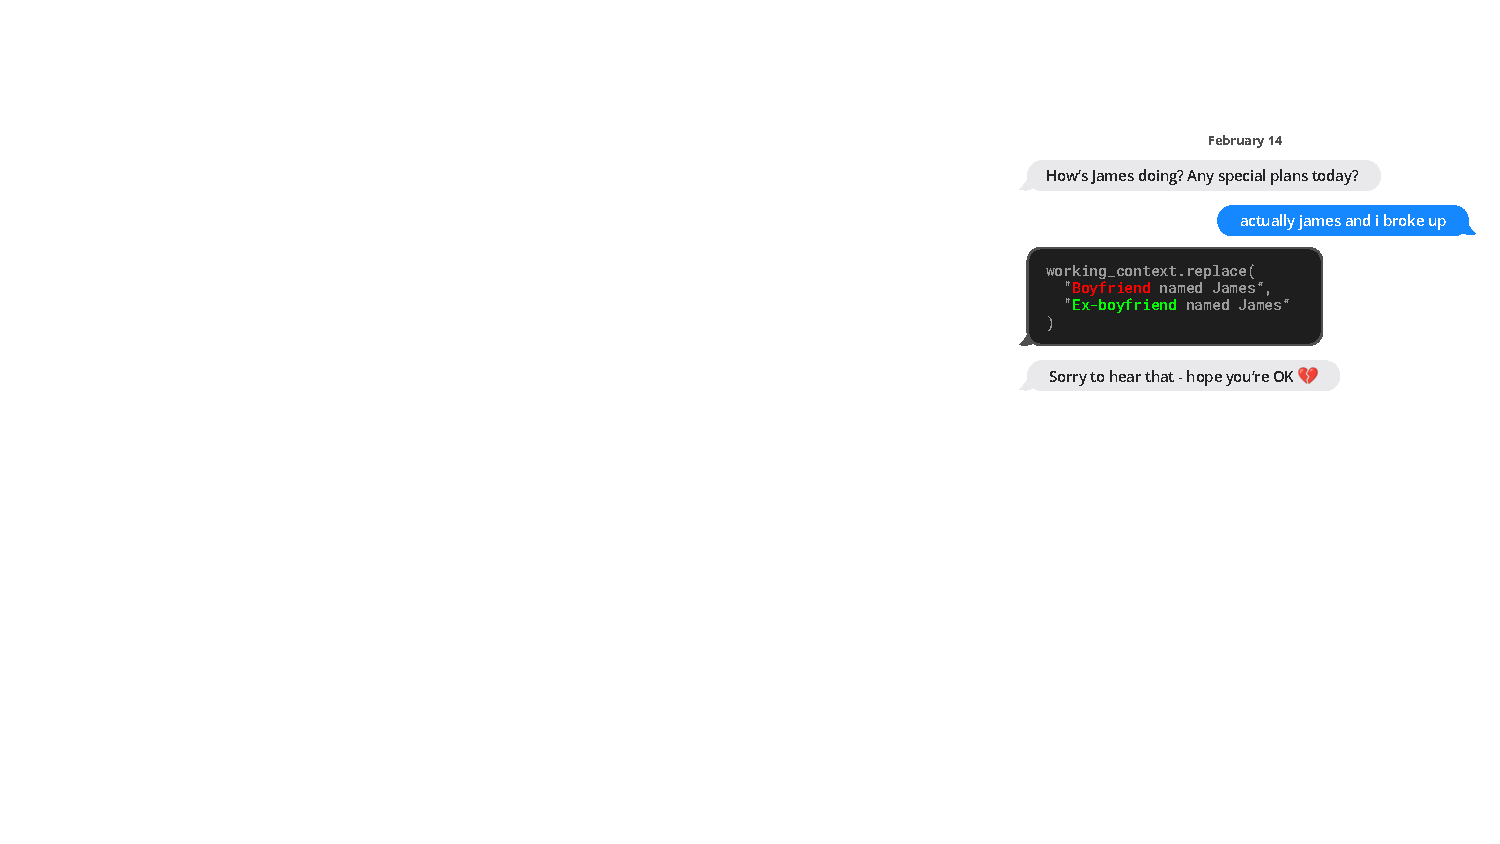
\includegraphics[width=0.45\textwidth]{images/memgpt_diagrams_wide_memory_correction.pdf}
\end{center}
    \caption{
An example conversation snippet where \ours (left) updates stored information. Here the information is stored in working context memory (located within the prompt tokens).
}
    \label{fig:example-memory-correction}
\end{figure}
